\documentclass{article} % For LaTeX2e
\usepackage{nips14submit_e,times}
\usepackage{hyperref}
\usepackage{url}
%\documentstyle[nips14submit_09,times,art10]{article} % For LaTeX 2.09

\usepackage{graphicx}
\usepackage{subfigure}
\usepackage{amsmath,amssymb}
\def\etal{{\textit{et~al.~}}}

\title{Supplement to \\
``Exploiting Linear Structure Within Convolutional Networks
  for Efficient Evaluation" \\
NIPS2014}


\newcommand{\fix}{\marginpar{FIX}}
\newcommand{\new}{\marginpar{NEW}}

\begin{document}

\maketitle

\section{Forward propagation time breakdown}
Table \ref{evaluation_time} shows the time breakdown of forward propagation for each layer in the CNN architecture we explored. Close to 90\% of the time is spent on convolutional layers, and within these layers the majority of time is spent on the first two. 

\begin{table}[h]
\small
\parbox{.5\linewidth}{
\centering
\begin{tabular}{rrr}
\hline
{\bf Layer} & {\bf Time per batch (sec)} & {\bf Fraction} \\
\hline
Conv1 & $2.8317 \pm 0.1030 $ & 21.97\% \\
MaxPool & $0.1059 \pm 0.0154$ & 0.82\% \\
LRNormal & $0.1918 \pm 0.0162$ & 1.49\% \\
Conv2 & $4.2626 \pm 0.0740 $ & 33.07\% \\
MaxPool & $0.0705  \pm 0.0029$ & 0.55\% \\
LRNormal & $0.0772\pm 0.0027$ & 0.60\% \\
Conv3 & $1.8689\pm 0.0577$ & 14.50\% \\
MaxPool & $0.0532\pm 0.0018 $ & 0.41\% \\
Conv4 & $1.5261\pm 0.0386$ & 11.84\% \\
Conv5 & $1.4222\pm 0.0416$& 11.03\% \\
MaxPool & $0.0102\pm 0.0006 $ & 0.08\% \\
FC & $0.3777\pm 0.0233$ & 2.93\% \\
FC & $0.0709  \pm 0.0038$ & 0.55\% \\
FC & $0.0168 \pm 0.0018$ & 0.13\% \\
Softmax & $0.0028 \pm 0.0015$ & 0.02\%\\
\hline 
Total & $12.8885$ & \\
\hline
\end{tabular}
}
\parbox{.5\linewidth}{
\centering
\begin{tabular}{rrr}
\hline
{\bf Layer} & {\bf Time per batch (sec)} & {\bf Fraction} \\
\hline
Conv1 & $0.0604 \pm 0.0112$ & 5.14\% \\
MaxPool & $0.0072 \pm 0.0040$ & 0.61\% \\
LRNormal & $0.0041 \pm 0.0043$ &  0.35\% \\
Conv2 & $0.4663 \pm 0.0072$ & 39.68\% \\
MaxPool & $0.0032 \pm 0.0000$ &  0.27\% \\
LRNormal & $0.0015 \pm 0.0003$ & 0.13\% \\
Conv3 & $0.2219 \pm 0.0014$ & 18.88\% \\
MaxPool & $0.0016 \pm 0.0000$ & 0.14\% \\
Conv4 & $0.1991 \pm 0.0001$ & 16.94\% \\
Conv5 & $0.1958 \pm 0.0002$ &  16.66\% \\
MaxPool & $0.0005  \pm 0.0001$ & 0.04\% \\
FC & $0.0077 \pm 0.0013$ & 0.66\% \\
FC & $0.0017 \pm 0.0001$ & 0.14\% \\
FC & $0.0007 \pm 0.0002$  & 0.06\% \\
Softmax & $0.0038 \pm 0.0098$ & 0.32\%\\
\hline 
Total & 1.1752 & \\
\hline
\end{tabular}
}
\caption{Evaluation time in seconds per layer on CPU (left)
  and GPU (right) with batch size of 128. Results are averaged over 8
  runs.} 
\label{evaluation_time}
\end{table}


\section{Theoretical speedups}
We can measure the theoretically achievable speedups for a particular approximation in term of the number of floating point operations required to compute the target output.
While it is unlikely that any implementation would achieve speedups equal to the theoretically optimal level, the number of necessary floating point operations still provides an informative upper bound on the gains.

Table \ref{table:mono_perf} shows the theoretical speedup of the monochromatic approximation. 
The majority of the operations result from the convolution part of the computation. 
In comparison, the number of operations required for the color transformation is negligible. 
Thus, the theoretically achievable speedup decreases only slightly as the number of color components used is increased. 

Figure \ref{fig:biclustering_theory} plots the theoretically achievable speedups against the drop in classification performance for various configurations of the biclustering with outer product decomposition technique.  
For a given setting of input and output clusters numbers, the performance tends to degrade as the rank is decreased. 

\begin{table}[t]
\small
\centering
\begin{tabular}{ccccc}
\hline
{\bf Number of colors} & & {\bf Increase in test error} & & {\bf Theoretical speedup}\\
& & & &\\
& {\bf Original} & {\bf $\|W\|_{data}$ distance metric} & {\bf Fine-tuned} & \\
\hline
4 & 24.1\% & 5.9\% & 1.9\% & 2.97$\times$ \\
6 & 16.1\% & 2.4\% & 0.4\% & 2.95$\times$ \\
8 & 9.9\% & 1.4\% & 0.2\% & 2.94$\times$\\
12 & 3.5\% & 0.7\% & 0\% & 2.91$\times$\\
16 & 1.99\% & 0.8\% & - & 2.88$\times$\\
24 & 1.43\% & 0.4\% & - & 2.82$\times$\\
\hline 
\end{tabular}
\caption{Performance when first layer weights are replaced with monochromatic approximation and the corresponding theoretical speedup. Classification error on ImageNet12 validation images tends to increase as the approximation becomes harsher (i.e. fewer colors are used). Theoretical speedups vary only slightly as the number of colors used increases since the color transformation contributes relatively little to the total number of operations.} 
\label{table:mono_perf}
\end{table}
\nocite{*}
\bibliographystyle{splncs}
\bibliography{bibliography}


\begin{figure}[t]
\centering
\begin{minipage}{0.75\textwidth}
  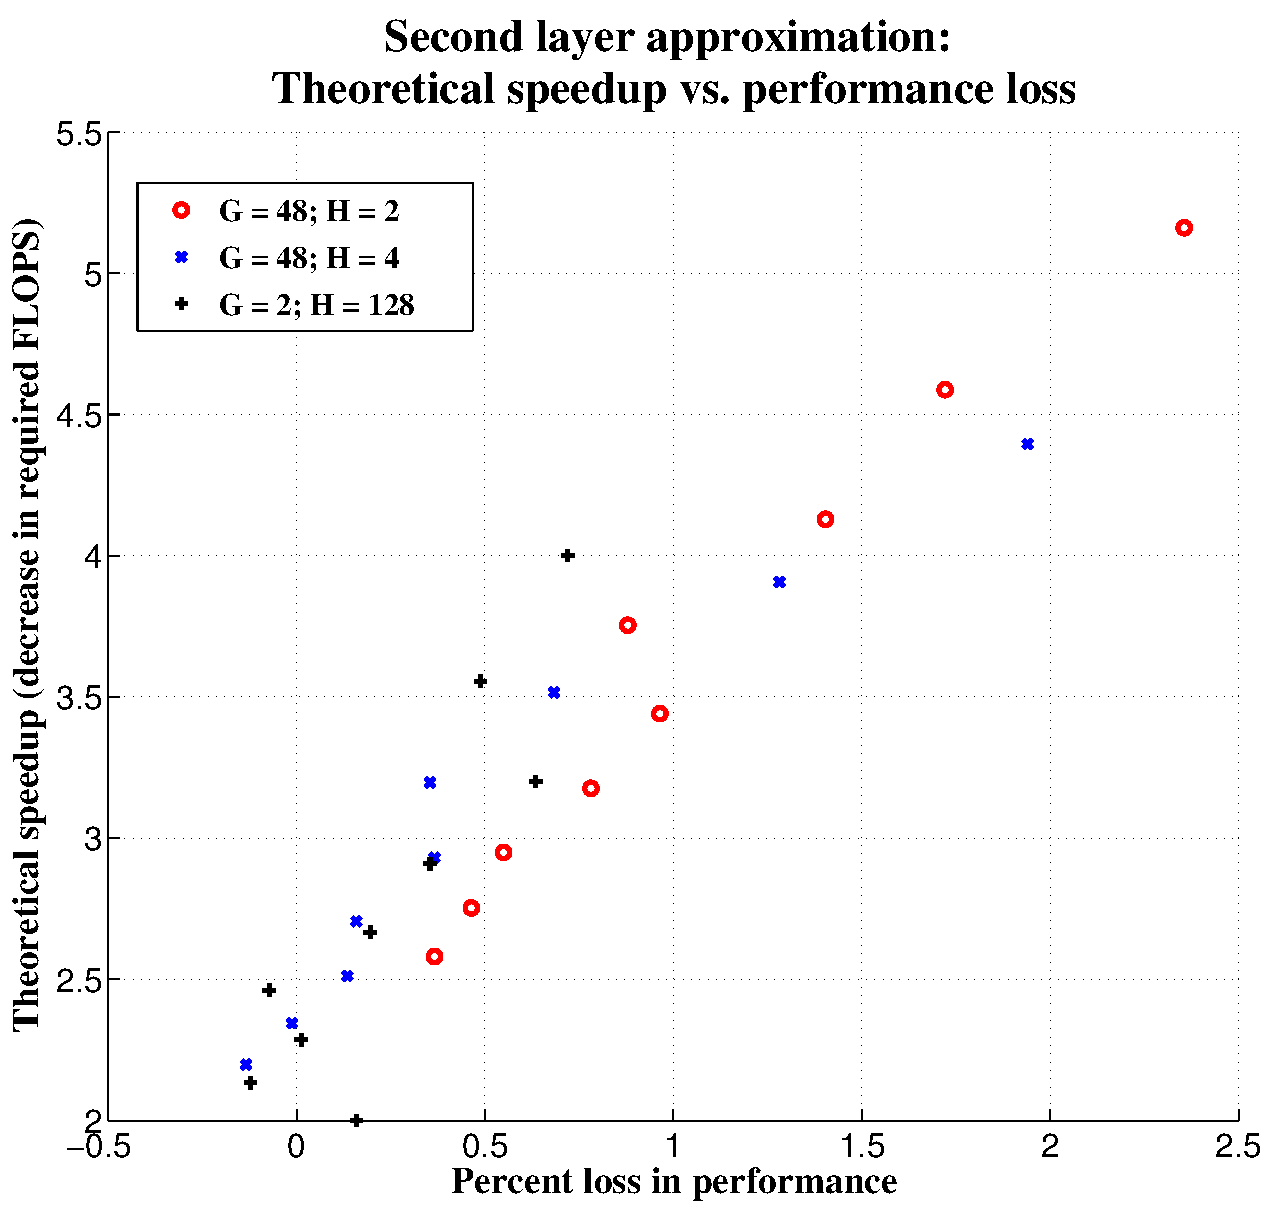
\includegraphics[width=\linewidth]{img/layer2_theoreticalspeedup_vs_performance_loss.pdf} 
\end{minipage}
\caption{Theoretically achievable speedups vs. classification error for various biclustering approximations.}
\label{fig:biclustering_theory}
\end{figure}


\end{document}
